\section{Plant Species}

A database is used to store all plant species and their associated properties which are used to determine their ability to grow in given environments and, subsequently, deduce a plausible distribution using the ecosystem simulator. Details about these, how they can be edited and new species added is discussed in \textit{Specie Properties} and  \textit{Storing Species} respectively.

\subsection{Specie Properties}

When configuring a new specie it is necessary to specify with it a set of properties which are used to link it to given suitable environments. These properties are discussed in detail below and summarized in table \ref{tab:specie_properties}.

\begin{table}[]
  \centering
	    \begin{tabular}{|p{4cm}|p{7cm}|p{2cm}|p{0cm}|}
		\hline	
		\textbf{Property} & \textbf{Value} & \textbf{Unit} \\
		\hline
		\textbf{Slope} & Maximum Slope & Degrees \\
		\hline
		\multirow{3}{*}{\textbf{Growth}} & \multicolumn{1}{l|}{Maximum canopy} & \multicolumn{1}{l|}{Centimetres} \\\cline{2-3}
        						   & \multicolumn{1}{l|}{Maximum root size} & \multicolumn{1}{l|}{Centimetres} \\\cline{2-3}
                               & \multicolumn{1}{l|}{Maximum height} & \multicolumn{1}{l|}{Centimetres} \\
		\hline
		\multirow{2}{*}{\textbf{Ageing}} & \multicolumn{1}{l|}{Start of decline} & \multicolumn{1}{l|}{Months} \\\cline{2-3}
        						   & \multicolumn{1}{l|}{Maximum age} & \multicolumn{1}{l|}{Months} \\
		\hline    
		\multirow{2}{*}{\textbf{Seeding}} & \multicolumn{1}{l|}{Maximum seeding distance} & \multicolumn{1}{l|}{Metres} \\\cline{2-3}
        						   & \multicolumn{1}{l|}{Annual seed count} & \multicolumn{1}{l|}{ - } \\
		\hline    
		\multirow{4}{*}{\textbf{Illumination}}
								& \multicolumn{1}{l|}{Start of prime} & \multicolumn{1}{l|}{hours} \\\cline{2-3}
								& \multicolumn{1}{l|}{End of prime} & \multicolumn{1}{l|}{hours} \\\cline{2-3}
								& \multicolumn{1}{l|}{Minimum} & \multicolumn{1}{l|}{hours} \\\cline{2-3}
								& \multicolumn{1}{l|}{Maximum} & \multicolumn{1}{l|}{hours} \\
		\hline   
		\multirow{4}{*}{\textbf{Humidity}}
								& \multicolumn{1}{l|}{Start of prime} & \multicolumn{1}{l|}{millimetres} \\\cline{2-3}
								& \multicolumn{1}{l|}{End of prime} & \multicolumn{1}{l|}{millimetres} \\\cline{2-3}
								& \multicolumn{1}{l|}{Minimum} & \multicolumn{1}{l|}{millimetres} \\\cline{2-3}
								& \multicolumn{1}{l|}{Maximum} & \multicolumn{1}{l|}{millimetres} \\
		\hline    
		\multirow{4}{*}{\textbf{Temperature}}
								& \multicolumn{1}{l|}{Start of prime} & \multicolumn{1}{l|}{degrees} \\\cline{2-3}
								& \multicolumn{1}{l|}{End of prime} & \multicolumn{1}{l|}{degrees} \\\cline{2-3}
								& \multicolumn{1}{l|}{Minimum} & \multicolumn{1}{l|}{degrees} \\\cline{2-3}
								& \multicolumn{1}{l|}{Maximum} & \multicolumn{1}{l|}{degrees} \\
		\hline                                                                           
		\end{tabular}
	\label{tab:specie_properties}	
\end{table}

\subsubsection{Slope}

Steep slopes cause essential water and soil nutrients to run-off, making them less rich and, therefore, less suited to plant growth. The slope angle also causes larger species to struggle to support their own biomass. For this reason, steeper slopes often cater for smaller plant species (grass, shrub, etc.). To model the effect of slope on given plant species, when configuring a new plant specie an associated \textit{maximum slope} must be specified.

\subsubsection{Growth}

To model the growth of a plant specie in the ecosystem simulator, it is necessary to specify: \textit{Maximum height}, \textit{maximum canopy width} and \textit{maximum root size}. Using this along with the specie's ageing properties (see \ref{subsubsec:ageing_properties}), it is possible to simulate the plants vertical growth (height), horizontal growth (canopy) and root coverage. Determining a plant's height and canopy width is also used to determine the shade it project's on other plants during the simulation. Modelling the plant's root growth is used to determine how far the plant can reach to fetch soil water. Note that a maximum canopy width of zero can be specified to model plants with no canopy.

\subsubsection{Ageing} \label{subsubsec:ageing_properties}

Biological life-cycle varies greatly between plant species. Whereas annual and biennials have a fixed lifespan of one and two years respectively, perennial plant species can live far longer. To model the life-cycle of different plant species they must be configured with an associated \textit{age of start of decline} and \textit{maximum age}. Using these two values, it is possible to simulate a plant getting weaker and, therefore, becoming more susceptible to domination from it's surrounding plants.

\subsubsection{Seeding}

It is necessary to replicate the spawning of offspring in the ecosystem simulator for two core reasons: 
\begin{enumerate}
\item \textit{Propagation}: Plants propagate on a terrain by producing new offspring which attempt to spawn and invade different areas. 
\item \textit{Succession}: New plants spawn to later succeed older and weaker plants of the same specie. 
\end{enumerate}

Depending on the specie, plants spawn new offspring by producing seeds or spores. Although biologically different, both can be considered identical for the sole purpose of modelling propagation and succession.\\

The number of seeds that a given plant creates annually is specie-dependent and therefore must accompany the specie's configuration.\\

Different species use different techniques to propagate their seeds. For example, some use fruit as a mechanism to propagate using animals digestive systems, some are coated with a sticky mucous to stick to the fur of animals passing by, some use the wind and some rely solely on gravity to take the seeds to the ground directly below. The seeding mechanism used directly affects the distance which can be achieved between parent and offspring and, to emulate this in the system, a \textit{maximum seeding distance} is configured.

\subsubsection{Illumination}

Illumination has a big impact on plant growth. Whereas some species strive in the shaded undergrowth, others require direct illumination all year round. To model this, the following illumination values must be configured with each plant specie:

\begin{itemize}
\item \textit{Minimum daily illumination}: The minimum daily illumination, in hours, at which a plant of this specie can survive.
\item \textit{Prime daily illumination range}: The daily illumination range, in hours, which is optimal for the given specie.
\item \textit{Maximum daily illumination}: The maximum daily illumination, in hours, at which a plant of this specie can survive.
\end{itemize}

\subsubsection{Humidity (rainfall)}

Soil water deposited into the soil by either rainfall or existing groundwater is absorbed by plant roots and is vital to its development and survival. Whereas some species have evolved to survive in arid climates with very little water, others require frequent downpours of rain. \\
To simplify water requirement specifications of different plant species, it is necessary to configure the amount of rainfall necessary as if this was the plant's only source of water (i.e no groundwater). The following values must be configured to grasp a species water requirements:

\begin{itemize}
\item \textit{Minimum monthly rainfall}: The minimum monthly rainfall, in millimetres, at which a plant of this specie can survive.
\item \textit{Prime monthly rainfall range}: The monthly rainfall range, in millimetres, which is optimal for the given specie.
\item \textit{Maximum monthly rainfall}: The maximum monthly rainfall, in millimetres, at which a plant of this specie can survive.\end{itemize}

\subsubsection{Temperature}

Another aspect of climates which greatly affect plant growth is temperature and, in order to model a specie's temperature requirements. the following values need to be configured:

\begin{itemize}
\item \textit{Minimum temperature}: The minimum temperature, in degrees, at which a plant of this specie can survive.
\item \textit{Prime temperature range}: The temperature range, in degrees, which is optimal for the given specie.
\item \textit{Maximum temperature}: The maximum temperature, in degrees, at which a plant of this specie can survive.
\end{itemize}

\subsection{Storing Species}

All species and associated properties are stored in a database for easy retrieval and filtering. A dedicated tool can be used to interact with the database to add or remove species and edit existing ones (see figure \ref{fig:plant_db_editor}).

\begin{figure}
\center
	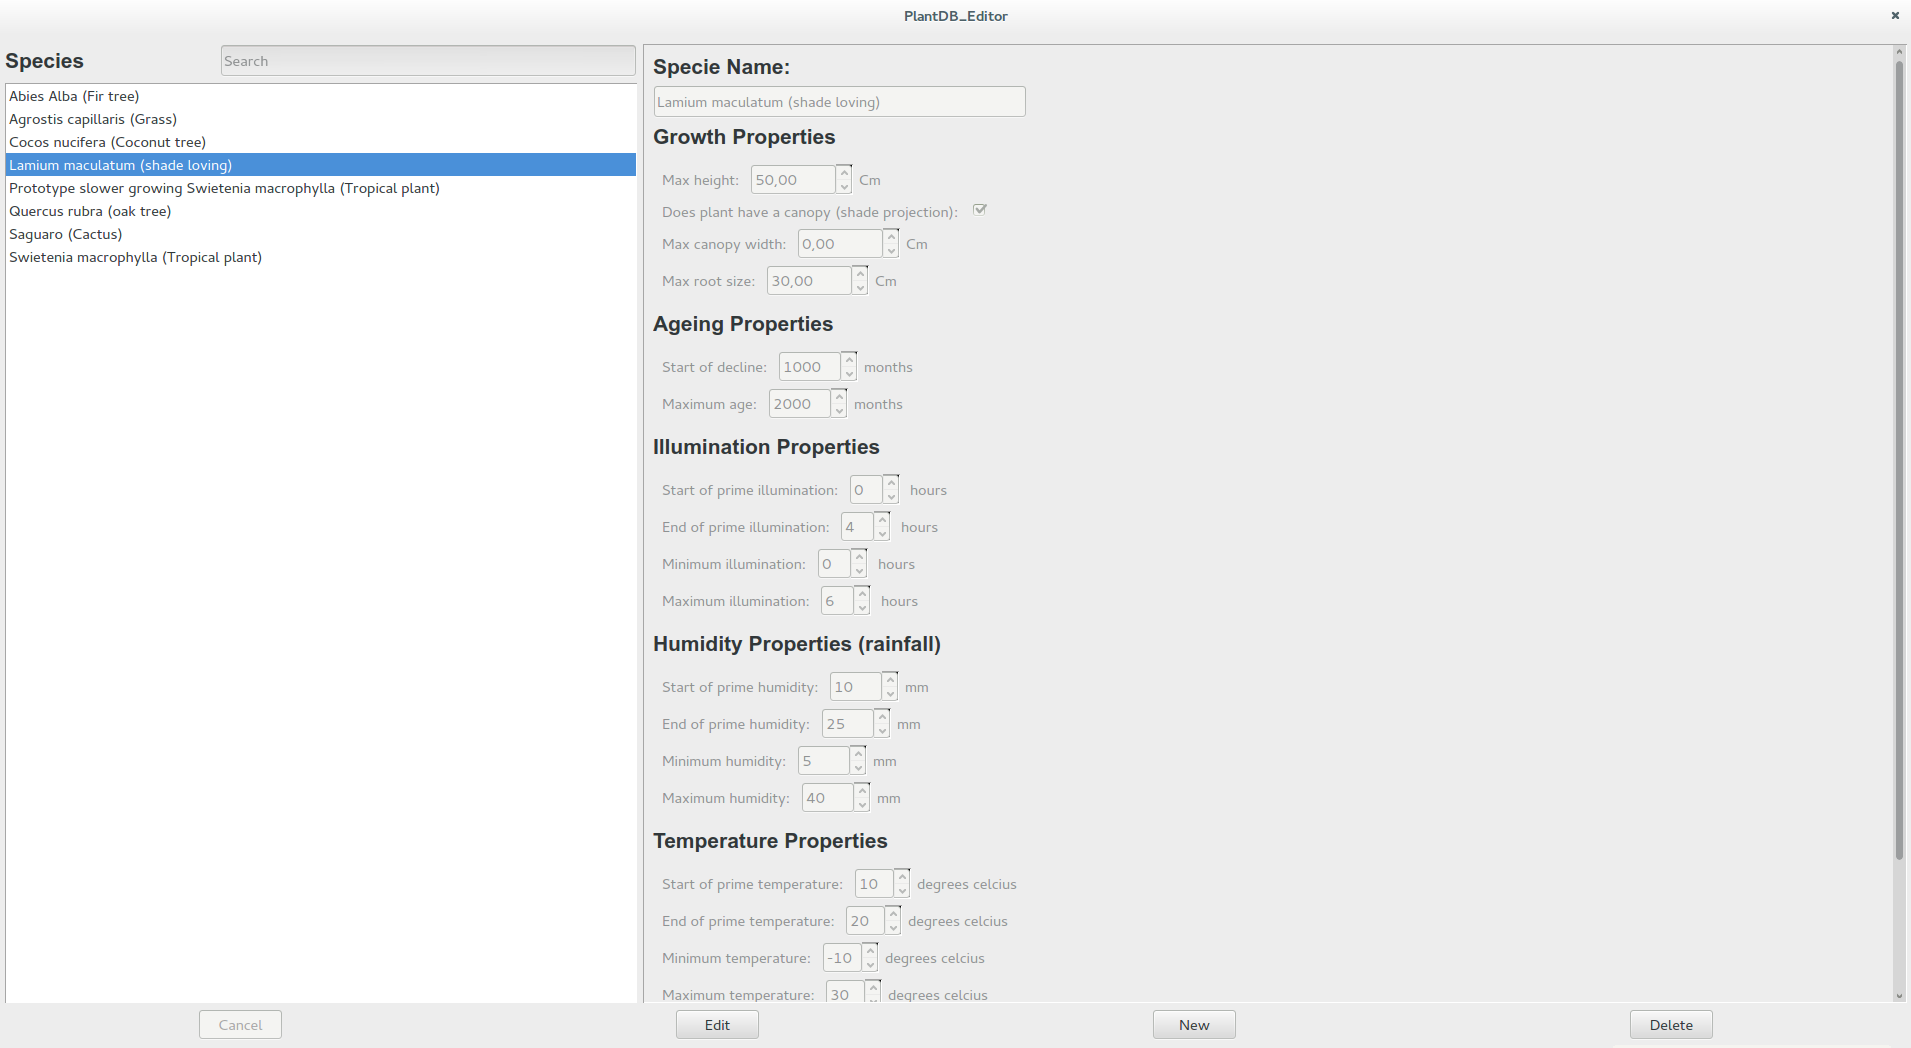
\includegraphics[width=\textwidth]{plant_db_editor.png}
	\caption{ Plant database editor tool.}	
	\label{fig:plant_db_editor}
\end{figure}
